\documentclass[border=40pt,varwidth]{standalone}% 

\usepackage{tikz}
\usetikzlibrary{shapes.geometric, arrows}

\tikzstyle{startstop} = [rectangle, rounded corners, 
minimum width=3cm, 
minimum height=1cm,
text centered, 
draw=black, 
fill=red!30]

\tikzstyle{io} = [trapezium, 
trapezium stretches=true, % A later addition
trapezium left angle=70, 
trapezium right angle=110, 
minimum width=3cm, 
minimum height=1cm, text centered, 
draw=black, fill=blue!30]

\tikzstyle{process} = [rectangle, 
minimum width=3cm, 
minimum height=1cm, 
text centered, 
text width=3cm, 
draw=black, 
fill=orange!30]

\tikzstyle{decision} = [diamond,
aspect = 2,
minimum width=1cm, 
minimum height=1cm, 
text centered, 
draw=black, 
fill=green!30]
\tikzstyle{arrow} = [thick,->,>=stealth]

\begin{document}
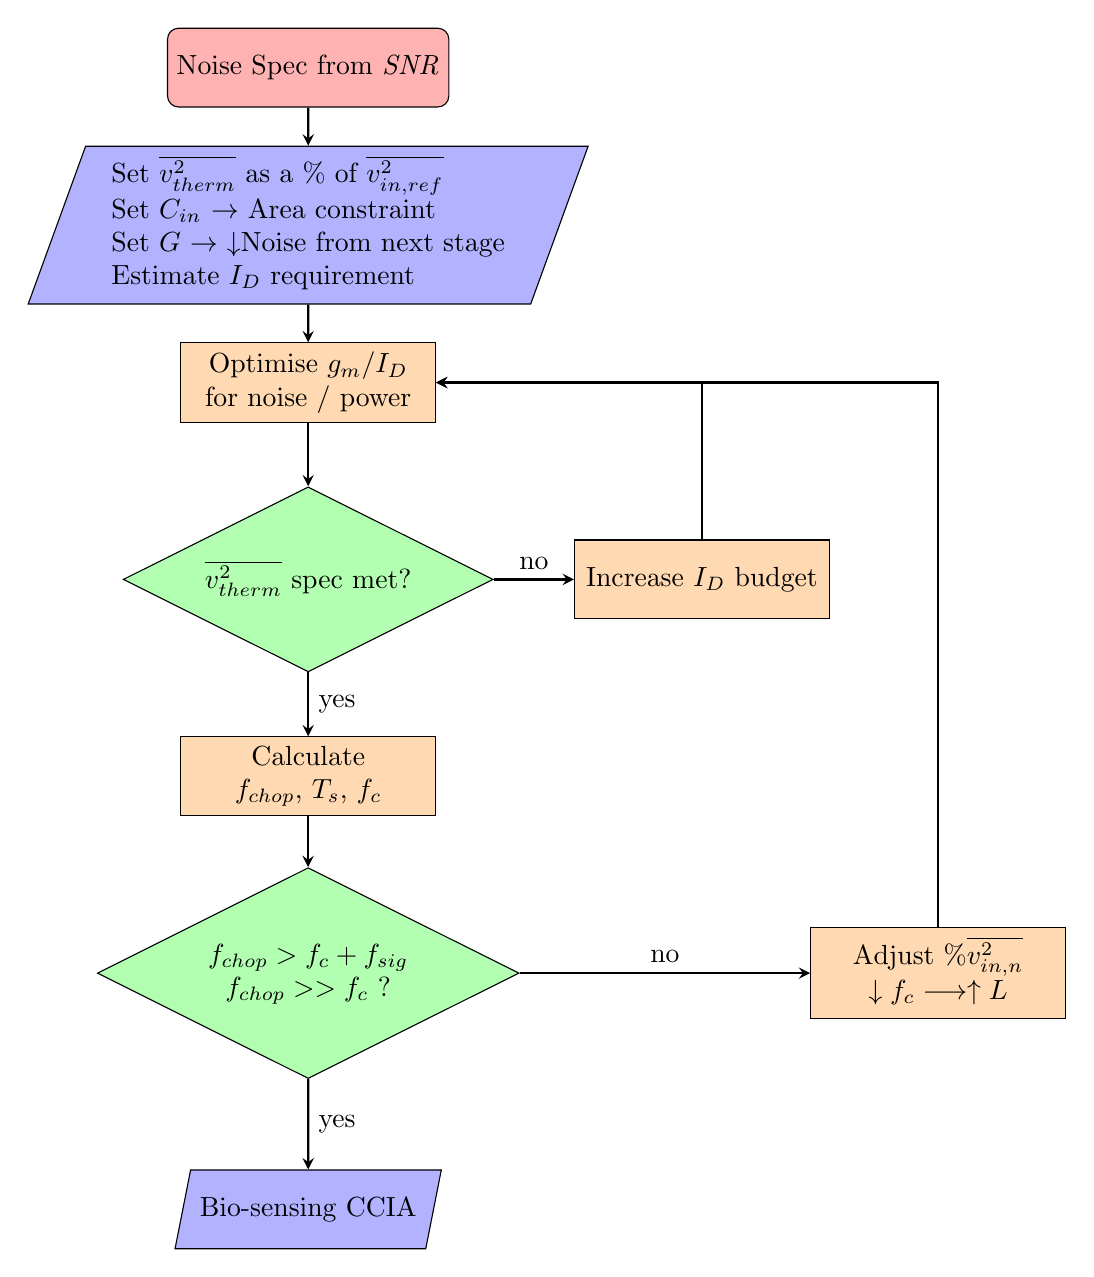
\begin{tikzpicture}[node distance=2cm]
  \node (start) [startstop] {Noise Spec from \textit{SNR}};
  \node (in1) [io, below of=start] {
  \begin{tabular}{l}
    Set $\overline{v^2_{therm}}$ as a $\%$ of $\overline{v_{in,ref}^2}$ \\
    Set $C_{in}$ $\rightarrow$ Area constraint \\ 
    Set $G$ $\rightarrow$  $\downarrow$Noise from next stage \\
    Estimate $I_D$ requirement
  \end{tabular}
  };
  \node (pro1) [process, below of=in1] {Optimise $g_m/I_D$ for noise / power};
  \node (dec1) [decision, below of=pro1, yshift = -0.5cm] {
    \begin{tabular}{c}
 %  $\overline{v^2_{therm}} \leq \%$ of $\overline{v_{in,ref}^2}$
   $\overline{v^2_{therm}}$ {spec}  {met?}
    \end{tabular}
    };
    \node (pro1b) [process, right of=dec1,xshift=3cm] {Increase $I_D$ budget};
  \node (pro2) [process, below of=dec1,yshift=-0.5cm] {Calculate $f_{chop}$, $T_s$, $f_{c}$};
    \node (dec2) [decision, below of=pro2, yshift = -0.5cm] {
    \begin{tabular}{c}
    $f_{chop}> f_{c} + f_{sig}$\\
    $f_{chop} >> f_{c}$ ?
    \end{tabular}
    };
    \node (pro2b) [process, right of=dec2, xshift=6cm] {
    \begin{tabular}{c}
    Adjust $\% \overline{v_{in,n}^2}$\\
    $\downarrow f_{c} \longrightarrow \uparrow L$
    \end{tabular}
    };
    \node (out) [io, below of=dec2, yshift = -1cm] {
    Bio-sensing CCIA
    };
    
    \draw [arrow] (start) -- (in1);
    \draw [arrow] (in1) -- (pro1);
    \draw [arrow] (pro1) -- (dec1);
    \draw [arrow] (dec1) -- node[anchor=south]{no} (pro1b);
    \draw [arrow] (dec1) -- node[anchor=west] {yes}(pro2);
    \draw [arrow] (pro2) -- (dec2);
    \draw [arrow] (dec2) -- node[anchor=south] {no}(pro2b);
    \draw [arrow] (pro2b) |- (pro1);
    \draw [arrow] (pro1b) |- (pro1);
    \draw [arrow] (dec2) -- node[anchor=west] {yes} (out);
\end{tikzpicture}
\end{document}